\documentclass{article}
\usepackage{mathtools}
\usepackage{listings}
\usepackage{qtree}
\usepackage{tikz-qtree}

\tikzset{
    black/.style={circle,draw=black,thick, minimum size=1.5em, inner sep=0},
    red/.style={circle,draw=red,thick, minimum size=1.5em, inner sep=0, fill=red!70},
    nil/.style={circle,fill=black, minimum size=0.5em, inner sep=0}
}
\begin{document}
\title{CS320 Homework 3}
\author{Dustin Randall}
\maketitle

\section{Construct RBT with the following keys: 21, 19, 17, 12, 15, 9}
\subsection*{Insert 21}
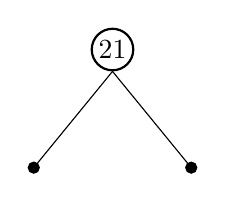
\begin{tikzpicture}[level/.style={sibling distance=20mm/#1}]
    \node [black] {21}
        child {[fill] circle (2pt)}
        child {[fill] circle (2pt)};
\end{tikzpicture} \\

\subsection*{Insert 19}
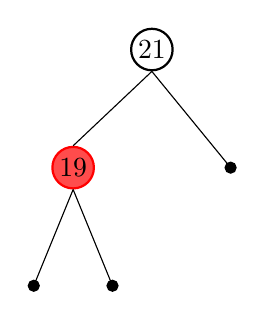
\begin{tikzpicture}[level/.style={sibling distance=20mm/#1}]
    \node[black]{21}
        child {node[red]{19}
            child {[fill] circle (2pt)}
            child {[fill] circle (2pt)}
        }
        child {[fill] circle (2pt)};
\end{tikzpicture} \\

\subsection*{Insert 17}
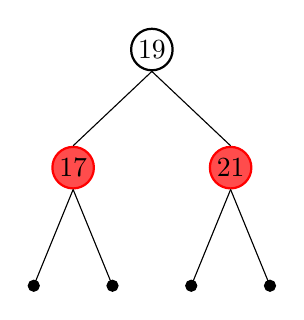
\begin{tikzpicture}[level/.style={sibling distance=20mm/#1}]
    \node[black]{19}
        child {node[red]{17}
            child {[fill] circle (2pt)}
            child {[fill] circle (2pt)}
        }
        child {node[red]{21}
            child {[fill] circle (2pt)}
            child {[fill] circle (2pt)}
        };
\end{tikzpicture} \\

\subsection*{Insert 12}
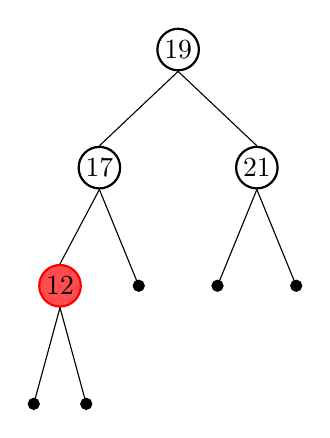
\begin{tikzpicture}[level/.style={sibling distance=20mm/#1}]
    \node[black]{19}
        child {node[black]{17}
            child {node[red]{12}
                child {[fill] circle (2pt)}
                child {[fill] circle (2pt)}
            }
            child {[fill] circle (2pt)}
        }
        child {node[black]{21}
            child {[fill] circle (2pt)}
            child {[fill] circle (2pt)}
        };
\end{tikzpicture} \\

\subsection*{Insert 15}
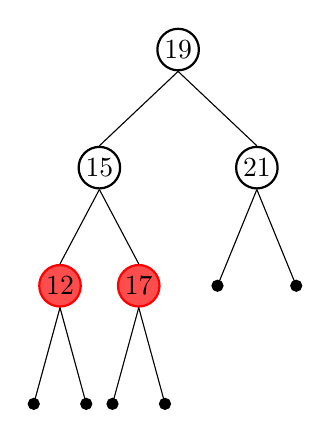
\begin{tikzpicture}[level/.style={sibling distance=20mm/#1}]
    \node[black]{19}
        child {node[black]{15}
            child {node[red]{12}
                child {[fill] circle (2pt)}
                child {[fill] circle (2pt)}
            }
            child {node[red] {17}
                child {[fill] circle (2pt)}
                child {[fill] circle (2pt)}
            }
        }
        child {node[black]{21}
            child {[fill] circle (2pt)}
            child {[fill] circle (2pt)}
        };
\end{tikzpicture} \\

\subsection*{Insert 9}

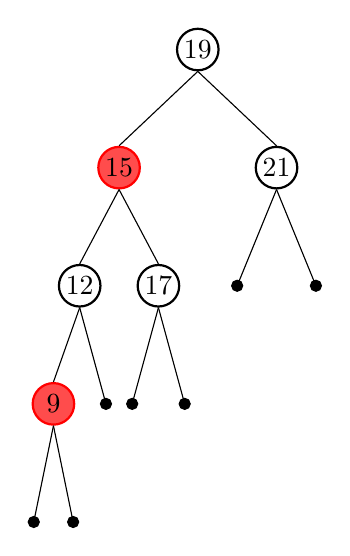
\begin{tikzpicture}[level/.style={sibling distance=20mm/#1}]
    \node[black]{19}
        child {node[red]{15}
            child {node[black]{12}
                child {node[red] {9}
                    child {[fill] circle (2pt)}
                    child {[fill] circle (2pt)}
                }
                child {[fill] circle (2pt)}
            }
            child {node[black] {17}
                child {[fill] circle (2pt)}
                child {[fill] circle (2pt)}
            }
        }
        child {node[black]{21}
            child {[fill] circle (2pt)}
            child {[fill] circle (2pt)}
        };
\end{tikzpicture} \\

\section{Delete the nodes of the RBT in the following order: 2, 5, 1, 14, 11, 15, 7, 8}
\subsection*{Initial Tree}
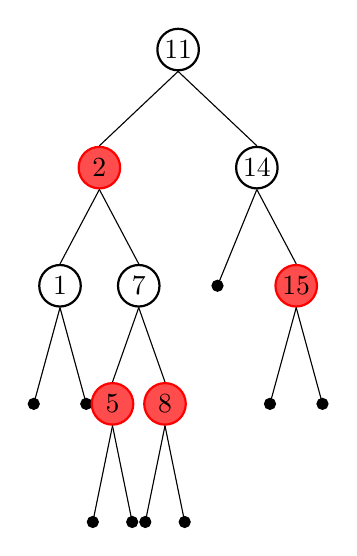
\begin{tikzpicture}[level/.style={sibling distance=20mm/#1}]
    \node[black]{11}
        child {node[red]{2}
            child {node[black]{1}
                child {[fill] circle (2pt)}
                child {[fill] circle (2pt)}
            }
            child {node[black]{7}
                child {node[red] {5}
                    child {[fill] circle (2pt)}
                    child {[fill] circle (2pt)}
                }
                child {node[red]{8}
                    child {[fill] circle (2pt)}
                    child {[fill] circle (2pt)}
                }
            }
        }
        child {node[black]{14}
            child {[fill] circle (2pt)}
            child {node[red]{15}
                child {[fill] circle (2pt)}
                child {[fill] circle (2pt)}
            }
        };
\end{tikzpicture} \\

\subsection*{Delete 2}
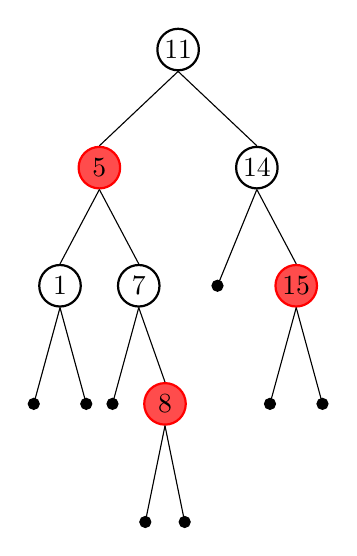
\begin{tikzpicture}[level/.style={sibling distance=20mm/#1}]
    \node[black]{11}
        child {node[red]{5}
            child {node[black]{1}
                child {[fill] circle (2pt)}
                child {[fill] circle (2pt)}
            }
            child {node[black]{7}
                child {[fill] circle (2pt)}
                child {node[red]{8}
                    child {[fill] circle (2pt)}
                    child {[fill] circle (2pt)}
                }
            }
        }
        child {node[black]{14}
            child {[fill] circle (2pt)}
            child {node[red]{15}
                child {[fill] circle (2pt)}
                child {[fill] circle (2pt)}
            }
        };
\end{tikzpicture} \\

\subsection*{Delete 5}
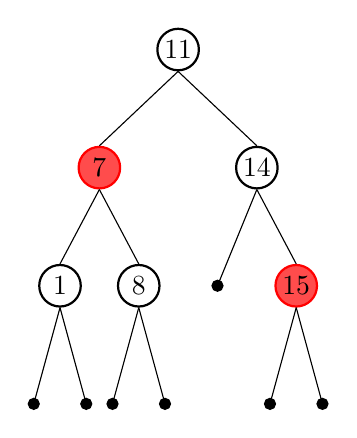
\begin{tikzpicture}[level/.style={sibling distance=20mm/#1}]
    \node[black]{11}
        child {node[red]{7}
            child {node[black]{1}
                child {[fill] circle (2pt)}
                child {[fill] circle (2pt)}
            }
            child {node[black]{8}
                child {[fill] circle (2pt)}
                child {[fill] circle (2pt)}
            }
        }
        child {node[black]{14}
            child {[fill] circle (2pt)}
            child {node[red]{15}
                child {[fill] circle (2pt)}
                child {[fill] circle (2pt)}
            }
        };
\end{tikzpicture} \\

\subsection*{Delete 1}
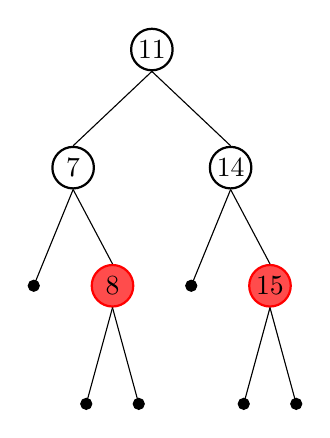
\begin{tikzpicture}[level/.style={sibling distance=20mm/#1}]
    \node[black]{11}
        child {node[black]{7}
            child {[fill] circle (2pt)}
            child {node[red]{8}
                child {[fill] circle (2pt)}
                child {[fill] circle (2pt)}
            }
        }
        child {node[black]{14}
            child {[fill] circle (2pt)}
            child {node[red]{15}
                child {[fill] circle (2pt)}
                child {[fill] circle (2pt)}
            }
        };
\end{tikzpicture} \\

\subsection*{Delete 14}
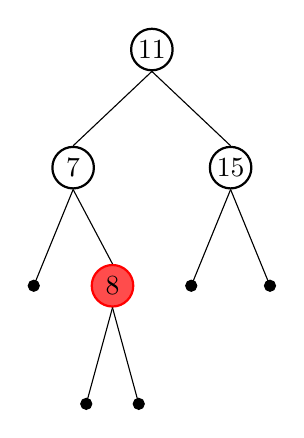
\begin{tikzpicture}[level/.style={sibling distance=20mm/#1}]
    \node[black]{11}
        child {node[black]{7}
            child {[fill] circle (2pt)}
            child {node[red]{8}
                child {[fill] circle (2pt)}
                child {[fill] circle (2pt)}
            }
        }
        child {node[black]{15}
            child {[fill] circle (2pt)}
            child {[fill] circle (2pt)}
        };
\end{tikzpicture} \\

\subsection*{Delete 11}
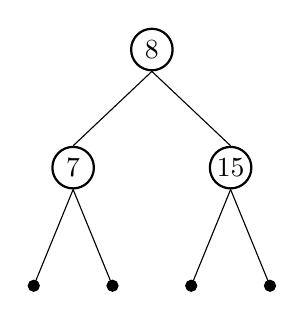
\begin{tikzpicture}[level/.style={sibling distance=20mm/#1}]
    \node[black]{8}
        child {node[black]{7}
            child {[fill] circle (2pt)}
            child {[fill] circle (2pt)}
        }
        child {node[black]{15}
            child {[fill] circle (2pt)}
            child {[fill] circle (2pt)}
        };
\end{tikzpicture} \\

\subsection*{Delete 15}
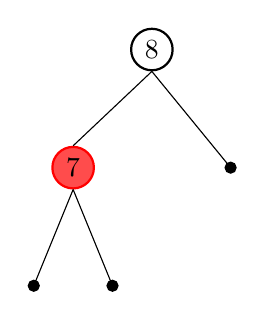
\begin{tikzpicture}[level/.style={sibling distance=20mm/#1}]
    \node[black]{8}
        child {node[red]{7}
            child {[fill] circle (2pt)}
            child {[fill] circle (2pt)}
        }
        child {[fill] circle (2pt)};
\end{tikzpicture} \\

\subsection*{Delete 7}
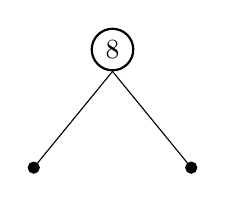
\begin{tikzpicture}[level/.style={sibling distance=20mm/#1}]
    \node[black]{8}
        child {[fill] circle (2pt)}
        child {[fill] circle (2pt)};
\end{tikzpicture} \\

\subsection*{Delete 8}
\end{document}